
\subsection{Graphe de retournement}

Le graphe de retournement est un concept utilisé dans le domaine des codes de Gray et des problèmes combinatoires.
Ce graphe est utilisé pour représenter les relations entre les objets combinatoires qui sont générés ou répertoriés par un code de Gray.
On appellera parfois retournement par flip, la notation anglaise. \newline

Dans un graphe de retournement, chaque sommet représente un objet combinatoire, comme une séquence de $n$-bits dans le cas des
codes de Gray sur des mots binaires de tailles $n$. Deux sommets sont reliés par une arête si les objets correspondants diffèrent
par une petite modification, souvent appelée "retournement", ce retournement correspond à une distance qui est appelée distance de
Hamming et est souvent égale à $1$. Par exemple, dans le contexte des codes de Gray, un retournement peut être l'inversion d'un seul
bit dans la séquence. Si le retournement est une opération réversible, c'est-à-dire qu'elle ramène l'objet initial à son état d'origine
lorsqu'elle est appliquée deux fois, le graphe de retournement est non dirigé. Un graphe de retournement offre une représentation
visuelle des relations entre les objets combinatoires générés par un code de Gray, ce qui facilite l'analyse et la compréhension
des propriétés et des comportements de ces codes. \newline

Voici par exemple le graphe de retournement des sous-ensemble de $\{1, 2, 3, 4, 5\}$ de taille $2$, aussi connu sous le nom de graphe
de Kneser pour $n=5$ et $k=2$, aussi noté $K(5, 2)$, deux sommets sont voisins si ils sont disjoints.

    {
        \centering
        \begin{center}
            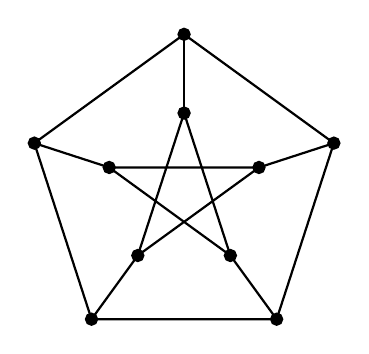
\begin{tikzpicture}[style=thick]
                \draw (18:2cm) -- (90:2cm) -- (162:2cm) -- (234:2cm) -- (306:2cm) -- cycle;
                \draw (18:1cm) -- (162:1cm) -- (306:1cm) -- (90:1cm) -- (234:1cm) -- cycle;
                \foreach \x in {18,90,162,234,306}{
                        \draw[fill=black] (\x:2cm) circle (2pt);
                        \draw[fill=black] (\x:1cm) circle (2pt);
                    }
                \foreach \x in {18,90,162,234,306}{
                        \draw (\x:1cm) -- (\x:2cm);
                    }
            \end{tikzpicture}
        \end{center}
        \par
    }

Le graphe de retournement associé au code de Gray pour une distance de Hamming de $1$ correspond à l'hypercube $\mathcal{Q}_n$,
une structure topologique importante en informatique parallèle et distribuée. Ainsi, les propriétés du graphe de retournement
fournissent des informations précieuses sur les relations entre les éléments du code de Gray et sur la structure de l'hypercube.\newline
